\documentclass[10pt, conference]{IEEEtran}
\IEEEoverridecommandlockouts
% The preceding line is only needed to identify funding in the first footnote. If that is unneeded, please comment it out.
\usepackage{cite}
\usepackage{amsmath,amssymb,amsfonts}
% \usepackage{algorithmic}
\usepackage{graphicx, wrapfig, subcaption}
\usepackage{textcomp}
\usepackage{xcolor}
\usepackage[numbers]{natbib} % Manual of natbib at https://gking.harvard.edu/files/natnotes2.pdf
\usepackage[hidelinks]{hyperref}
\usepackage[OT1]{fontenc}
\usepackage{setspace}
\begin{document}

\newcommand{\polimi}{Polytechnic University of Milan}
\newcommand{\deib}{Deparment of Electronics, Information and Bioengineering}

\title{Spy Your Mate\\
{\small Project Report --- 054327 Wireless Internet $\mid$ 054323 Internet of Things}
% \thanks{Identify applicable funding agency here. If none, delete this.}
}

\author{\IEEEauthorblockN{Davide Giacomini}
\IEEEauthorblockA{\textit{\polimi\space(PoliMi)} \\
\textit{\deib}\\
\textit{Milan (MI), Italy} \\
\textit{\today} \\
% giacomini.davide@outlook.com
}
% \\
% \IEEEauthorblockN{Jake Campbell}
% \IEEEauthorblockA{\textit{dept. of Engineering} \\
% \textit{University of Illinois at Chicago (UIC)}\\
% Chicago (IL), USA \\
% jacobpmcampbell@gmail.com}
% \and
% \IEEEauthorblockN{Sem Belay}
% \IEEEauthorblockA{\textit{dept. of Engineering} \\
% \textit{University of Illinois at Chicago (UIC)}\\
% Chicago (IL), USA \\
% sbelay2@uic.edu}
% \\
% \IEEEauthorblockN{Alejandro Dorvall}
% \IEEEauthorblockA{\textit{dept. of Engineering} \\
% \textit{University of Illinois at Chicago (UIC)}\\
% Chicago (IL), USA \\
% adorva2@uic.edu}
% \and
% \IEEEauthorblockN{5\textsuperscript{th} Given Name Surname}
% \IEEEauthorblockA{\textit{dept. name of organization (of Aff.)} \\
% \textit{name of organization (of Aff.)}\\
% City, Country \\
% email address or ORCID}
% \and
% \IEEEauthorblockN{6\textsuperscript{th} Given Name Surname}
% \IEEEauthorblockA{\textit{dept. name of organization (of Aff.)} \\
% \textit{name of organization (of Aff.)}\\
% City, Country \\
% email address or ORCID}
}

\maketitle
\thispagestyle{plain}
\pagestyle{plain}
% \onehalfspacing

\begin{abstract}
    After a global pandemic, video streaming calls have become the normality in every situation. Even though the major providers usually encrypt the traffic, some information can be extracted by the packets that are sent between the parties through the internet. By aggregating the packets of a conversation and analyzing some of their features through a ML algorithm, we can infer if somebody is present in front of the camera or there is nobody.
\end{abstract}

\section{Introduction}
In this report I am going to illustrate the work done for the joint project of Wireless Internet and Internet of Things.

I was required to extract some information from a video call with a provider of my choice. In particular, I was requested to analyze the traffic generated by a webcam call and, from such traffic, identify whether a person or only the background is recorded in the video. I was asked to capture the network traffic and filter all the video call packets. Subsequently, I had to extract some important features from the captured packets, and use those features to train a model of Machine Learning. Finally, I had to predict the presence of a person in the background using the trained model and compare the prediction with the ground truth. For the comparison, I had to use a Node-RED chart.

You can find all my code on GitHub\footnote{\href{https://github.com/davide-giacomini/spy_your_mate}{github.com/davide-giacomini/spy\_your\_mate}}. It has three folders that divide everything between Node-RED, Python and Latex (for this report).

\begin{table*}[t]
    \centering
    \begin{tabular}{| c ||c c c c||}
     \hline
      & Zoom IP Address & Zoom UDP Port & Local IP Address & Local UDP Port \\
     \hline\hline
     Capture 1 & 149.137.11.203 & 8801 & 192.168.1.15 & 60235 \\ 
     \hline
     Capture 2 & 149.137.11.142 & 8801 & 192.168.1.15 & 51541 \\
     \hline
     Capture 3 & 149.137.10.223 & 8801 & 192.168.1.15 & 52409 \\ 
     \hline
    \end{tabular}
    \caption{Addresses for each capture.}
    \label{table:table-addresses}
\end{table*}

\begin{figure*}[t]
    \centering
    \begin{subfigure}[b]{.33\linewidth}
        \centering
        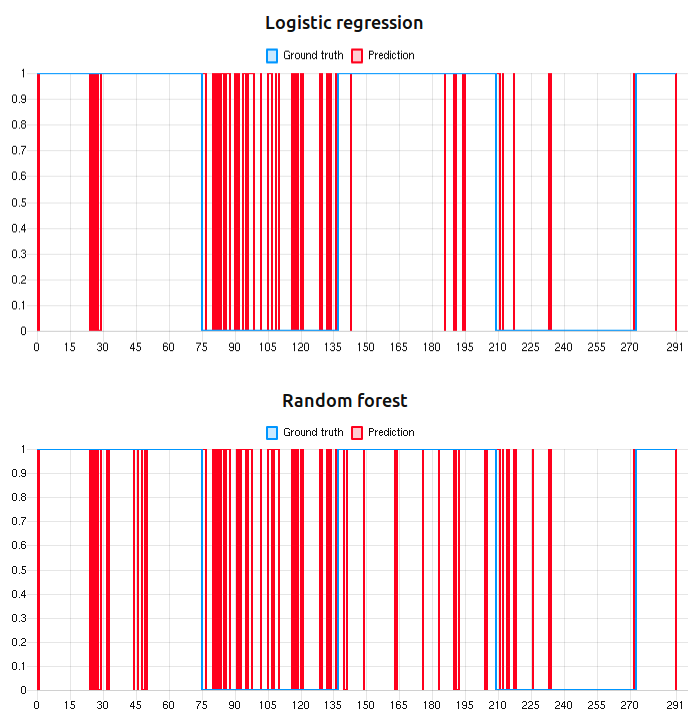
\includegraphics[width=\linewidth]{resources/prediction_with_basic_features_cropped.png}
        \caption{First Attempt}
        \label{fig:chart-first-attempt}
    \end{subfigure}%
    \begin{subfigure}[b]{.33\linewidth}
        \centering
        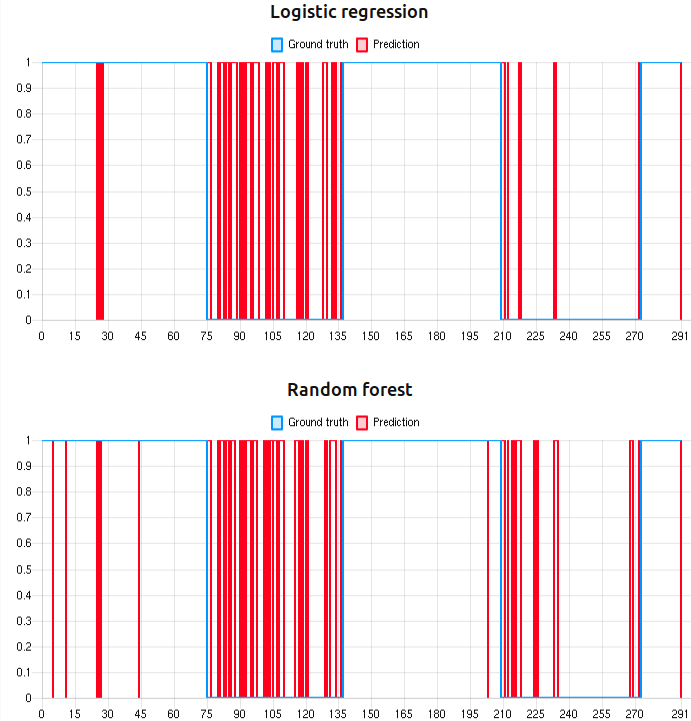
\includegraphics[width=\linewidth]{resources/prediction_with_inbound_and_outbound_features_cropped.png}
        \caption{Second Attempt}
        \label{fig:chart-second-attempt}
    \end{subfigure}
    \begin{subfigure}[b]{.33\linewidth}
        \centering
        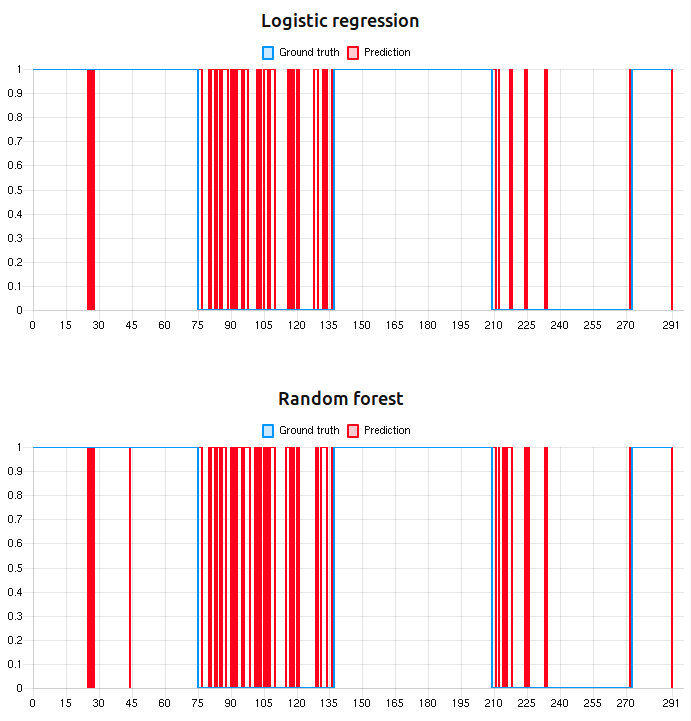
\includegraphics[width=\linewidth]{resources/prediction_with_inbound_and_outbound_features_bitrate_cropped.png}
        \caption{Last Attempt}
        \label{fig:chart-third-attempt}
    \end{subfigure}
    \caption{Node-RED charts for comparison with ground truth}
    \label{fig:charts-node-red}
\end{figure*}

\begin{figure*}[t]
    \centering
    \begin{subfigure}[b]{.5\linewidth}
        \centering
        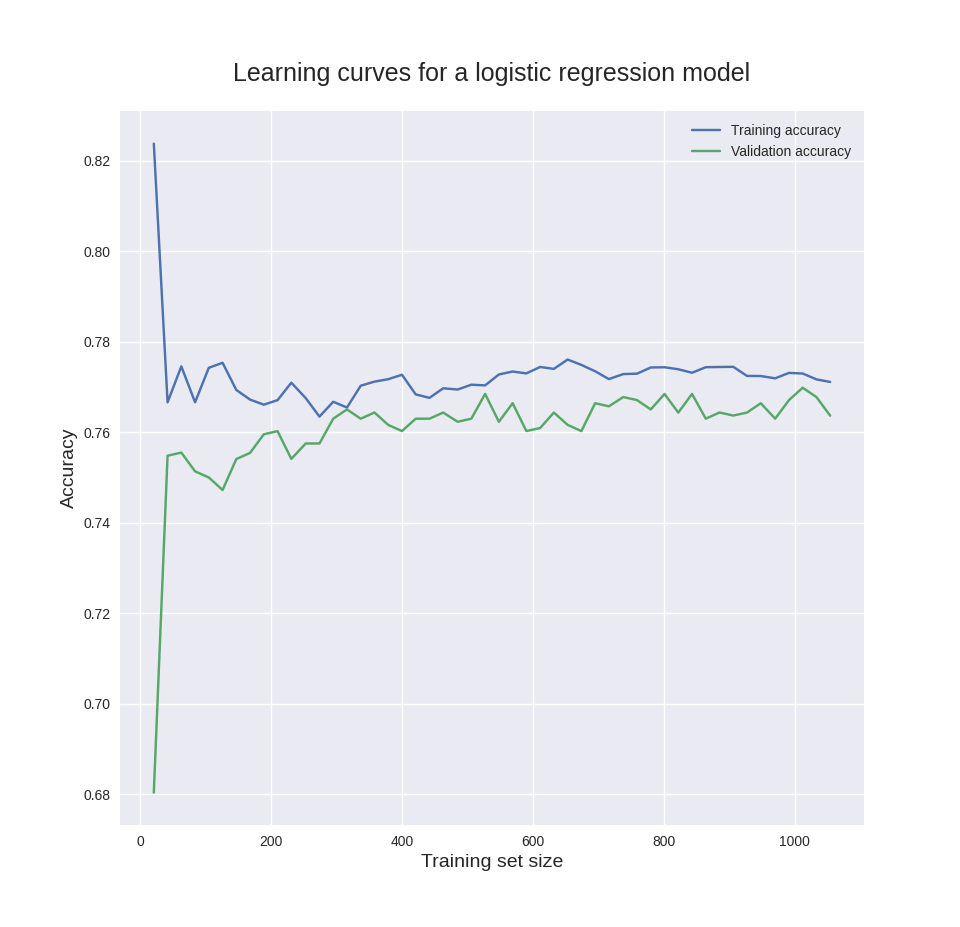
\includegraphics[width=\linewidth]{resources/learning_curve_basic_features_log_regr.png}
        \caption{Logistic Regression Curve}
        \label{fig:learning-curves-first-attempt-randfor}
    \end{subfigure}%
    \begin{subfigure}[b]{.5\linewidth}
        \centering
        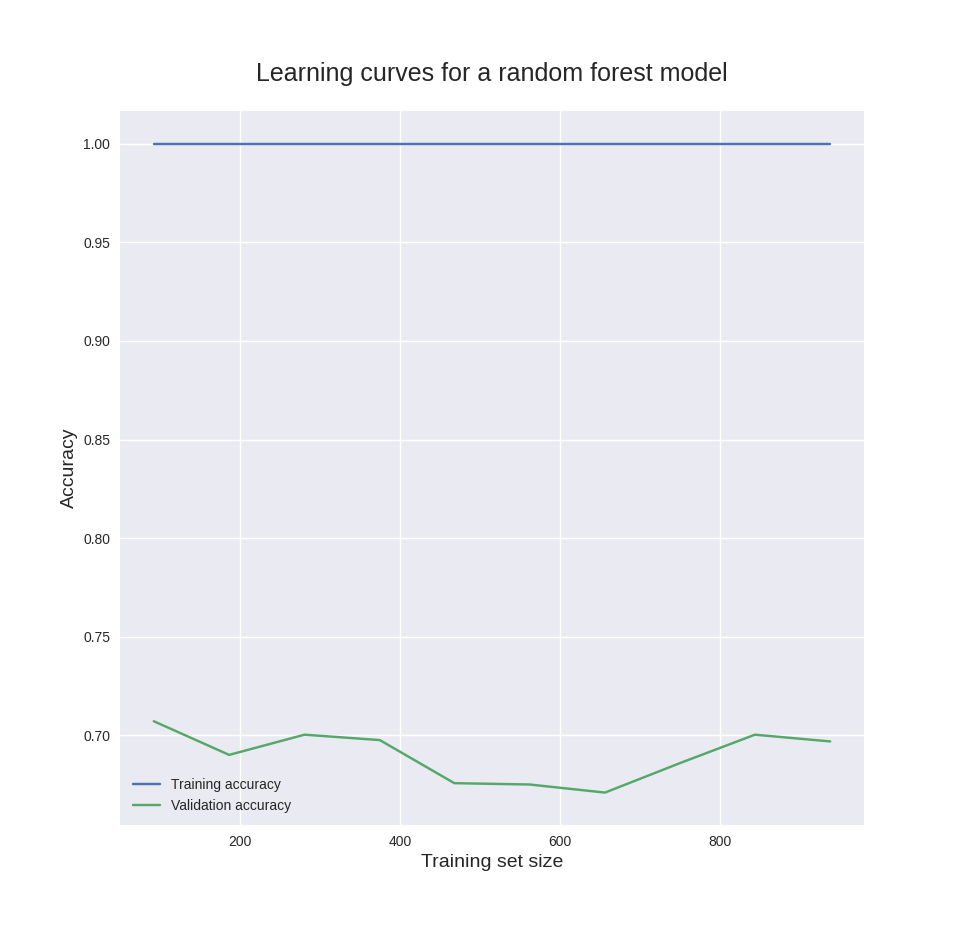
\includegraphics[width=\linewidth]{resources/learning_curve_basic_features_rand_for.png}
        \caption{Random Forest Curve}
        \label{fig:learning-curves-first-attempt-logreg}
    \end{subfigure}
    \caption{Learning curves in the first attempt}
    \label{fig:learning-curves-first-attempt}
\end{figure*}

\begin{figure*}[t]
    \centering
    \begin{subfigure}[b]{.45\linewidth}
        \centering
        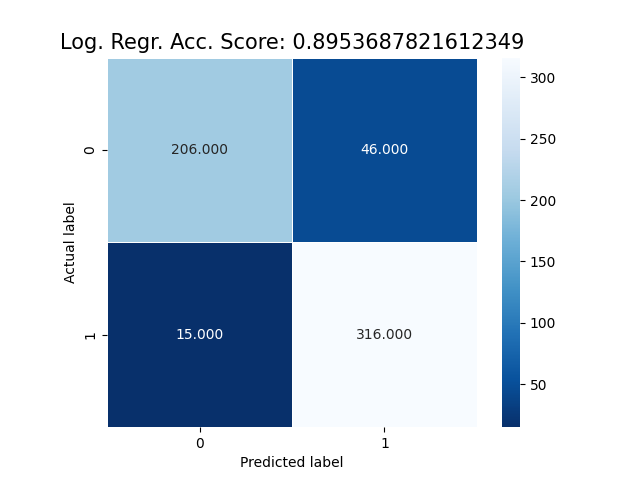
\includegraphics[width=\linewidth]{resources/confusion_matrix_basic_features_logreg.png}
        \caption{Logistic Regression Confusion Matrix}
        \label{fig:confusion-matrix-first-attempt-randfor}
    \end{subfigure}%
    \begin{subfigure}[b]{.45\linewidth}
        \centering
        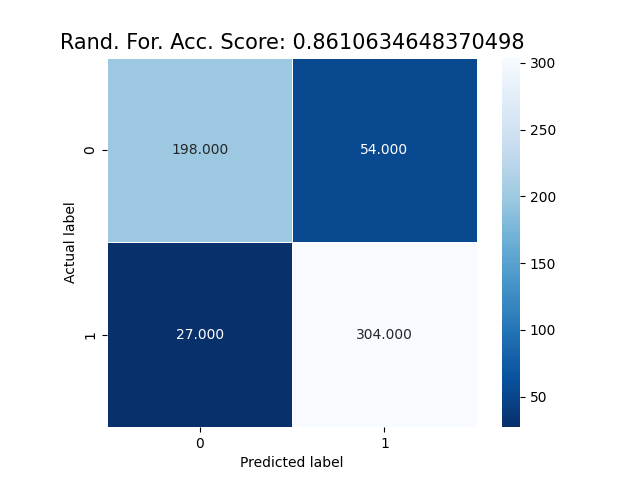
\includegraphics[width=\linewidth]{resources/confusion_matrix_basic_features_randfor.png}
        \caption{Random Forest Confusion Matrix}
        \label{fig:confusion-matrix-first-attempt-logreg}
    \end{subfigure}
    \caption{Confusion matrices in the first attempt}
    \label{fig:confusion-matrix-first-attempt}
\end{figure*}

\begin{figure*}[t]
    \centering
    \begin{subfigure}[b]{.5\linewidth}
        \centering
        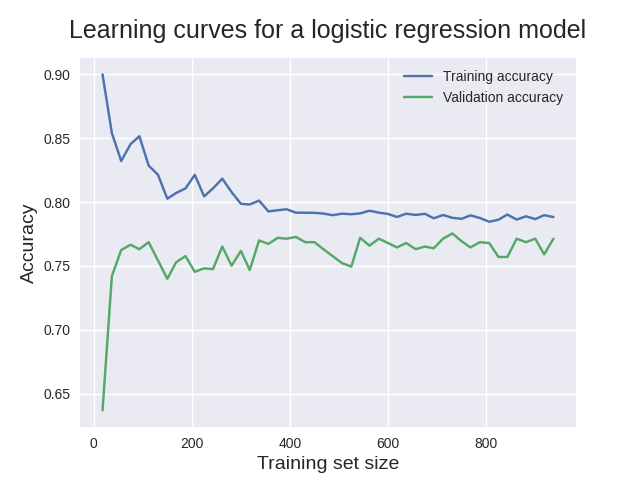
\includegraphics[width=\linewidth]{resources/learning_curve_in-out_features_log_regr.png}
        \caption{Logistic Regression Curve}
        \label{fig:learning-curves-second-attempt-randfor}
    \end{subfigure}%
    \begin{subfigure}[b]{.5\linewidth}
        \centering
        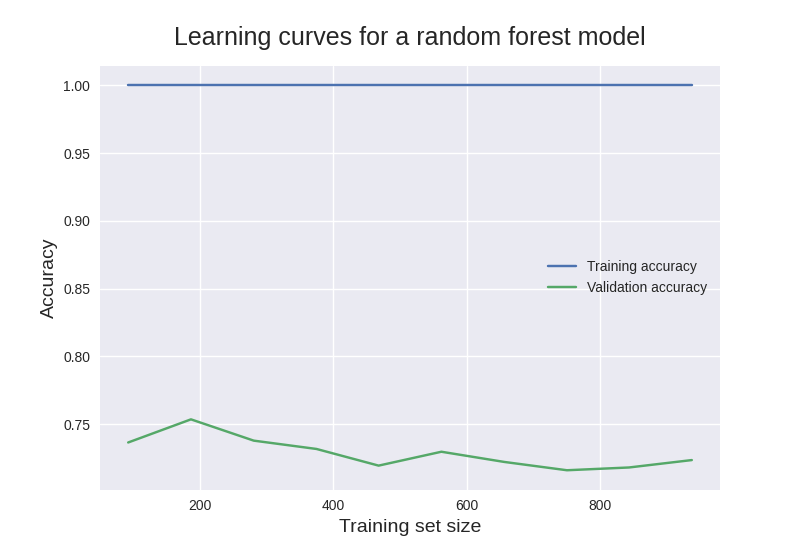
\includegraphics[width=\linewidth]{resources/learning_curve_in-out_features_rand_for.png}
        \caption{Random Forest Curve}
        \label{fig:learning-curves-second-attempt-logreg}
    \end{subfigure}
    \caption{Learning curves in the second attempt}
    \label{fig:learning-curves-second-attempt}
\end{figure*}

\begin{figure*}[t]
    \centering
    \begin{subfigure}[b]{.45\linewidth}
        \centering
        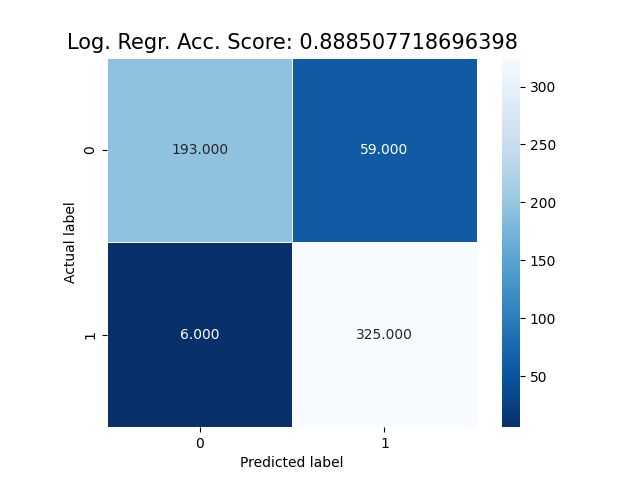
\includegraphics[width=\linewidth]{resources/confusion_matrix_in-out_features_logreg.png}
        \caption{Logistic Regression Confusion Matrix}
        \label{fig:confusion-matrix-second-attempt-randfor}
    \end{subfigure}%
    \begin{subfigure}[b]{.45\linewidth}
        \centering
        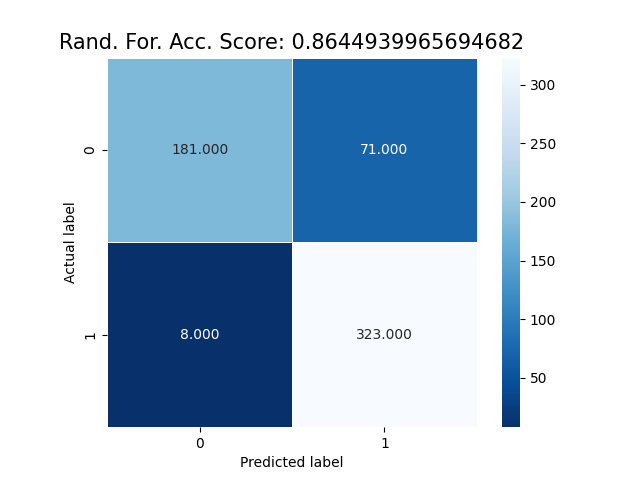
\includegraphics[width=\linewidth]{resources/confusion_matrix_in-out_features_randfor.png}
        \caption{Random Forest Confusion Matrix}
        \label{fig:confusion-matrix-second-attempt-logreg}
    \end{subfigure}
    \caption{Confusion matrices in the second attempt}
    \label{fig:confusion-matrix-second-attempt}
\end{figure*}

\begin{figure*}[t]
    \centering
    \begin{subfigure}[b]{.5\linewidth}
        \centering
        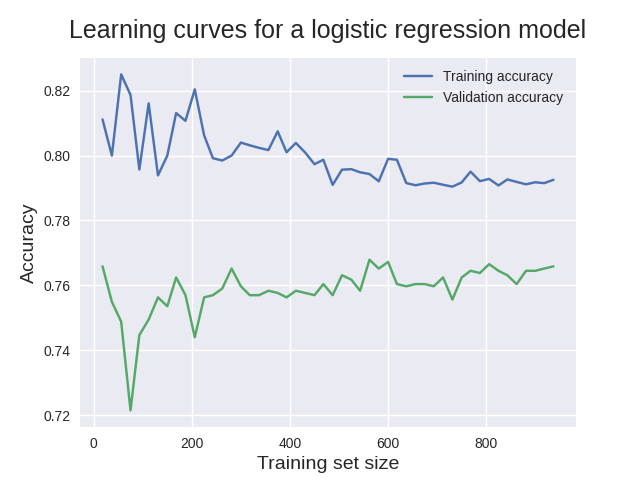
\includegraphics[width=\linewidth]{resources/learning_curve_in-out_features_bitrate_log_regr.png}
        \caption{Logistic Regression Curve}
        \label{fig:learning-curves-last-attempt-randfor}
    \end{subfigure}%
    \begin{subfigure}[b]{.5\linewidth}
        \centering
        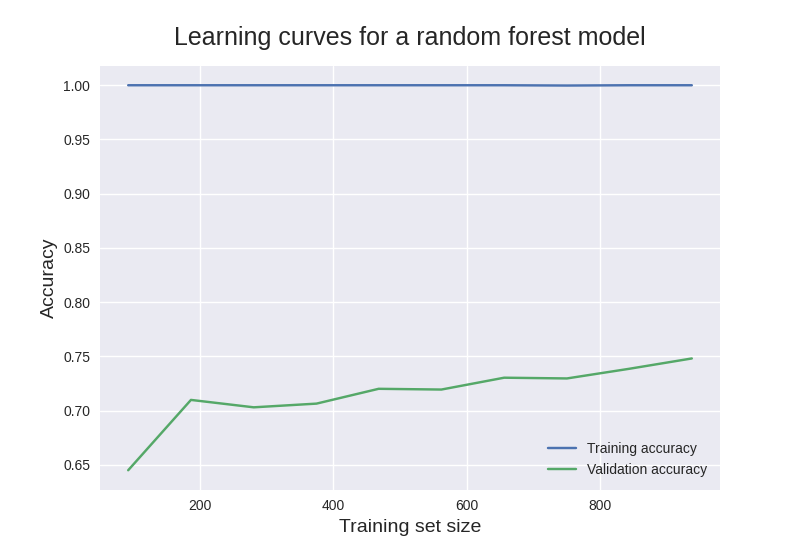
\includegraphics[width=\linewidth]{resources/learning_curve_in-out_features_bitrate_randfor.png}
        \caption{Random Forest Curve}
        \label{fig:learning-curves-last-attempt-logreg}
    \end{subfigure}
    \caption{Learning curves in the last attempt}
    \label{fig:learning-curves-last-attempt}
\end{figure*}

\begin{figure*}[t]
    \centering
    \begin{subfigure}[b]{.45\linewidth}
        \centering
        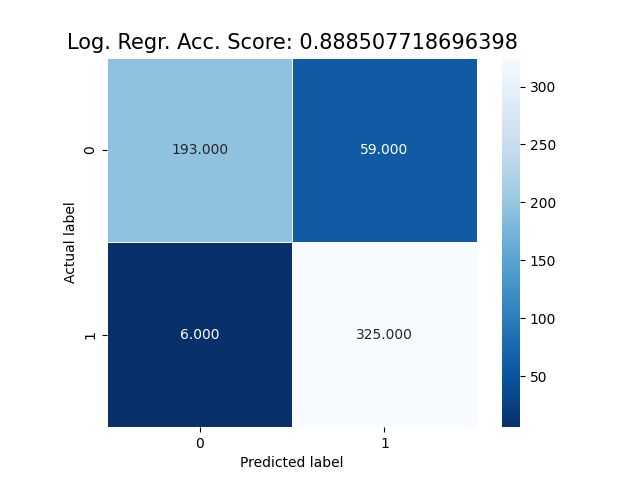
\includegraphics[width=\linewidth]{resources/confusion_matrix_in-out_features_bitrate_logreg.png}
        \caption{Logistic Regression Confusion Matrix}
        \label{fig:confusion-matrix-last-attempt-randfor}
    \end{subfigure}%
    \begin{subfigure}[b]{.45\linewidth}
        \centering
        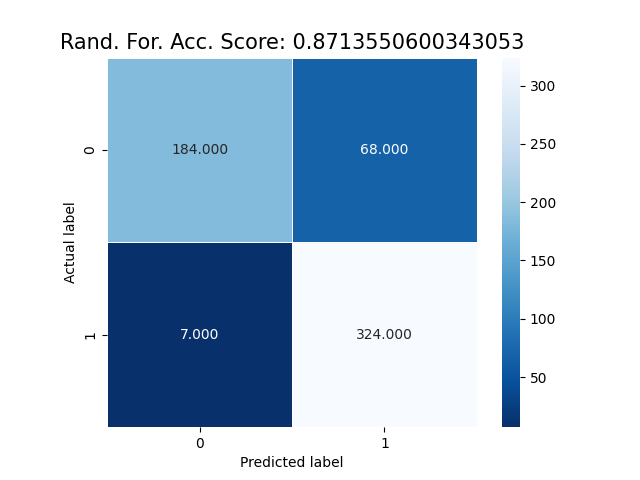
\includegraphics[width=\linewidth]{resources/confusion_matrix_in-out_features_bitrate_randfor.png}
        \caption{Random Forest Confusion Matrix}
        \label{fig:confusion-matrix-last-attempt-logreg}
    \end{subfigure}
    \caption{Confusion matrices in the last attempt}
    \label{fig:confusion-matrix-last-attempt}
\end{figure*}

\section{Method}

The first step was to choose a software for network traffic, hence I chose Wireshark\footnote{\href{https://www.wireshark.org/}{wireshark.org}}. I recorded three vide calls. In the first one I was alone, in the other two I was with another person (different each time). The captures duration is more or less between 300 seconds and 420 seconds. For the video calls I used my laptop (Asus) and my smartphone (Samsung Galaxy S10). The provider I used was Zoom\footnote{\href{https://zoom.us/}{zoom.us}}, as I am comfortable with it.

I needed both the IP addresses and the UDP ports to filter the packets of the video call. In Wireshark there is a convenient window under \texttt{Statistics -> Conversations} which shows you the conversations based on the chosen protocol. Clicking on \texttt{UDP}, I ordered the conversations in order to highlight the one with the highest number of packets (and bytes) transferred. It was easy to see which one is the actual video call, because there is a difference of several orders of magnitude in number of bytes exchanged. The addresses and the ports that I extracted from Wireshark can be seen at Table~\ref{table:table-addresses}.


\subsection{Python Code}
After extracting the addresses, I used them to filter out only the packets regarding the conversation between the parties. I used PyShark\footnote{\href{https://pypi.org/project/pyshark/}{pypi.org/project/pyshark/}} to manipulate the captures. The Python scripts are used to extract the packets, organize them in chunks of half a second, and save the chunks and their features on a csv file, later used for training or testing. The scripts are called in order by the \texttt{prepare\_*.py} scripts. I divided them for convenience during debugging.

The training and testing is done by two scripts called \texttt{script\_ML\_*.py}. The cross validation is only used to understand if the features chosen are good to make an accurate prediction, and the second script is used to actually predict the results. I used the second capture (\texttt{capture2\_test.csv}) to test the model and the other two captures to train it.

I incrementally added features to get a model each time more accurate, and I finally ended up with (TODO NUMBER OF FEATURES) features. Each of them represents a chunk of half a second packets. I am going to describe them below. Notice that each point represents three features, i.e. inbound packets, outbound packets and all packets:
\begin{itemize}
    \item Average packet interval: the average time between one packet and the next.
    \item Average packet size: the average packet size in bytes.
    \item Packets number: the total number of packets.
    \item Bit rate: the number of bytes per half a second.
    \item TODO: more features
\end{itemize}

I used two different algorithms to train the model: logistic regression and random forest. The predictions are saved as \texttt{csv} files to be later used in Node-RED.

\subsection{Node-RED Flow}
In Node-RED I was required to compare the ground truth with the actual prediction done in Python.

In order to do that, I read with Node-RED two different csv files (the capture file exported in csv and the prediction of python) and compared the results with the Chart of Node-RED. For comparing the results, I had to filter out the ground truth taking only the multiples of half a second. The prediction file, instead, had already been prepared with Python.

\subsection{ML Training and Testing}
For the training and the testing of models (both logistic regression and random forest), I divided the work in two main parts. The former one is the cross validation, to understand more or less the accuracy of my predictions, and the latter one is the actual training and prediction with the features I chose during the cross validation. Both the cross validation and the actual training and prediction take as input the \texttt{capture*.csv} files that I prepared with PyShark. I used \texttt{scikit-learn}\footnote{\href{https://scikit-learn.org/stable/}{scikit-learn.org/stable/}} for the ML methods.

The cross validation file (\texttt{script\_ML\_cross\_validation.py}) takes as input the csv files thought for the training part (I chose capture 1 and 3 for the training part) and applies a K fold cross validation with $k=5$. I set the maximum training set size to the 80\% of the training data, hence the minimum validation set is 20\% of the training data. I am basing the terminology on the slide number 5 from the set of slides \cite{matteucci2022neuralnetworkstraining}. After the cross validation, a learning curve shows the training and validation accuracy in function of the number of samples (training size).

After the cross vaildation, we can proceed with the actual training of the model and the subsequent prediction with the trained model. The steps are two: the training and then the testing. For the training, as before, the file takes as input the csv training files and trains the two models (logistic regression and random forest) with those two files. Then, for the testing, the file takes as input the csv file of capture 2 and predicts the presence or absence of a person in front of the webcam. The prediction is then exported in a csv file for Node-RED and is also compared to the ground truth, showing the confusion matrix and the accuracy of the prediction.

\section{Experimental Results}

I ran several trials, but I will report here only the ones that I found interesting for the sake of the document.

\subsection{First attempt}
I started with five features: average packets interval, average packets size, inbound and outbound packets number, total packets number.

\subsubsection{Cross validation results}

The learning curve of the cross validation for both models can be seen at Fig.~\ref{fig:learning-curves-first-attempt}. Notice that the training curve of the random forest is always equal to 100\% accuracy, and that is not exactly the best behaviour required (Fig.~\ref{fig:learning-curves-first-attempt-randfor}). Nonetheless, the validation accuracy is quite consistent with the testing results, which I will show later. In particular, the validation accuracy stands at around 70\%. On the other hand, the logistic regression curve is quite ``normal'' (Fig.~\ref{fig:learning-curves-first-attempt-logreg}). The training accuracy is about 77\% and the validation accuracy is about 76\%.

\subsubsection{Training and testing results}

After the prediction, the Python script shows a confusion matrix and the accuracy for each model. You can see both confusion matrices and accuracies at Fig.~\ref{fig:learning-curves-first-attempt}. You can notice that the model predicts relatively well when the person is actually in front of the webcam (output 1), but it cannot predict very well when there is only background (output 0). After exporting the predicted results to the csv file, I used Node-RED to read from that file and compare it to the ground truth. The results of the comparison are shown in a Node-RED chart, that I am reporting here at Fig.~\ref{fig:chart-first-attempt}. As we noticed with the confusion matrices, the models get a better result when there is actually a person in front of the camera. In this precise case, the random forest model is very dirty and not very useful.

\subsection{Second attempt}
For this second attempt, I added some features based on the precedent ones, dividing though inbound and outbound packets. In particular, I added: average inbound and outbound packets interval, average inbound and outbound packets size.

\subsubsection{Cross validation results}


The learning curve here got a little better for the random forest model. As we can see at Fig.~\ref{fig:learning-curves-second-attempt}, the training curve for the logistic regression model stands at around 78\%, the validation curve for the same model stands at around 76\% and the validation curve for the other model is around 72\% (2\% more than the first attempt). As always, the training curve of the random forest model is not informative, as it always stays at 100\%.

\subsubsection{Training and testing results}

We can see from Fig.~\ref{fig:confusion-matrix-second-attempt} how the prediction of the presence of a person has got better again, expecially comparing the matrices to the ones at Fig.~\ref{fig:confusion-matrix-first-attempt}. Although, the background recognition is still a problem. If we take a look at the chart of Fig.~\ref{fig:chart-second-attempt}, we can see how now the situation got better expecially for the random forest model. We can basically see that, apart from one or two problems, the prediction of the presence of a person is basically accurate for both models.

\subsection{Last attempt}
For the last attempt, I added the bit rate for inbound, outbound and all the packets.

\subsubsection{Cross validation results}

I could still increase the validation accuracy for the random forest model. At Fig.~\ref{fig:learning-curves-last-attempt} we can see the different values. The training and validation curves of the logistic regression model reciprocally stands at around 79\% and 76\%, and the validation curve of the random forest model is 74\%.

\subsubsection{Training and testing results}

The confusion matrices at Fig.~\ref{fig:confusion-matrix-last-attempt} shows that there is relatively no difference between the previous attempt, but the charts at Fig.~\ref{fig:chart-third-attempt} show a very little improvement in the cleanness of the prediction. Unfortunately, although the last background interval is predicted quite well, especially with the logistic regression model, the first one is not predicted at all.

\subsection{Failed attempts}

I will not report here the several attempts that are not worth the time of reading, but I wanted to consider a particular case.

I told you that I divided the packets in chunks of half a second, but it is not the only possibility. The rules of the project required to divide the packets in chunks between 100ms and 900ms, hence I also tried to change the interval, for example with 250ms of interval. Although the number of samples was increased (because of the shorter interval), this seemed to be useless from the point of view of training the models. Instead, it seemed to degrade the predictions, especially of the logistic regression model.
\section{Conclusion}
We proposed a solution for overcoming the problems that were issued by the Covid-19.

The doctor is actually able to test if the patient could be ill without even the need to touch them with their hand (Figure \ref{fig:doctor}).

We are proud to have shared with you our work.

\begin{figure}[t]
    \centering
    \includegraphics[width=\linewidth]{resources/doctor-diagnosis.jpg}
    \caption{A doctor that diagnose a patient}
    \label{fig:doctor}
\end{figure}
\section{Further Improvements}

This work could be improved with a better and bigger dataset, in order to try different combinations of captures. Moreover, I think that if there are some valid features that I missed in my work, it could be a strong improvement even without amplifying the dataset.

Moreover, I was unfortunately alone and I did not try to make a real video call, instead I called myself between laptop and smartphone. Considering the local Wifi network, the only external information the algorithm can extract is the one coming from the Zoom server and not from the other endpoint of the communication. I did however involved other people during the call, in order to have some data with more than one person in front of the camera. I although strongly believe that, overall, this work can be improved with a better environment.


\bibliographystyle{unsrtnat} % Cannot upload \bibliographystyle{IEEEtran}, don't know why
\bibliography{bibliography}

\end{document}
